\scanpage{121}
composantes irréductibles de $Z$ qui sont de codim 1 dans $X$. Alors $g$ est \uline{entier} sur $\underline{\mathcal O}_X$.

\uline{Lemme 2} Soit \deleted{$X$ \unsure{comme dessus}, $f$} \deleted{$X,f$ \unsure{comme}} $X$ \deleted{loc} préschéma \deleted{\unsure{f}} réduit, $f$ section de $\underline{\mathcal O}_X$ non diviseur de 0, \inserted{et \deleted{\unsure{tel}} telle que $\underline{\mathcal O}_X/f$ réduit}, $g$ une section de $\underline{\mathcal O}_X$ sur $X_f$, entière sur $\underline{\mathcal O}_X$ en tant que \deleted{section} pseudo-\deleted{sect.}fonction rat. sur $X$. Alors $g$ est partout définie.

\figure{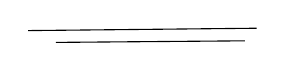
\begin{tikzpicture}[x=1cm,y=1cm]
\draw (0,.15)--(2.9,.18);\draw (.35,0)--(2.75,.02);
\end{tikzpicture}}

\uline{Corollaire 1} Dans les conditions de la proposition, soit $g$ une fonction rationnelle sur $X$. Pour que $g$ soit une section de $\underline{\mathcal O}_X^*$, il f. et s. que $g|X_f$ le soit, et que \deleted{$g$} les $g_{y_i}\in\underline{\mathcal O}_{\unsure{y_i}}^*$. \deleted{\unsure{pour}}
\margin{$\longrightarrow$}

\uline{Corollaire 2} Diagramme exact
\diagram{\begin{tikzcd}
\Gamma(X_f,\underline{\mathcal O}_{X_f}^*) \arrow[r] & \mathbf{Z}^I \\
\Gamma(X,\underline{\mathcal O}_X^*)\times\mathbf{Z} \arrow[u] \arrow[r] & \mathbf{Z} \arrow[u]
\end{tikzcd}}
\margin{120}
